\subsubsection{Hadronisation mechanisms for c and b quarks}

Brief intro to fragmentation vs recombination

describe recombination implementations with references,
also statistical hadronisation?

effects of hadronisation on yields, pT spectrum, v2

Available RHIC and LHC data (no figures)

Discuss also Bs and Bc, see e.g. arXiv:hep-ph/0004041

\subsubsection{Measurement performance studies (ALICE and CMS)}

Simulation studies for the measurement of the $D_s$, $\Lambda_c$ and $\Lambda_b$
production were carried out by the ALICE Collaboration~\cite{ITSTDR} and are updated in the present document. A projection of the performance for the $B_s$ meson by the CMS Collaboration is also reported~\cite{CMSFTR2017}. The $D_s$, $\Lambda_c$ and $\Lambda_b$ ($\to\Lambda_c\pi$) reconstruction strongly benefits from the improved track spatial resolution of the ALICE Inner Tracking System Upgrade, because they have small mean proper decay lengths (e.g.\,about 60~$\mu$m for $\Lambda_c$)
and large combinatorial backgrounds. The $\Lambda_c$, $\Lambda_b$ and $B_s$, in particular, require very large integrated luminosities, because the decay branching ratios are very small (e.g.\,about $3\times 10^{-4}$ for $\Lambda_b\to\Lambda_c(\to pK\pi)\pi$) and the combinatorial background is very large, in case for the $\Lambda_c$, which has a small separation from the interaction vertex and lower invariant-mass than the b-hadrons. In~\cite{CMSFTR2017} it has been shown that the statistical uncertainty in the lowest accessible $\pt$ intervals for these hadrons would increase above 20--30\% with integrated luminosity significantly lower than 10~nb$^{-1}$.

Figure~\ref{fig:HFDsBs} shows the projected performance for the $R_{\rm AA}$ of $D_s$ (left) and $B_s$ (right), compared with the corresponding non-strange mesons. The predicted difference between the $D^0$ and $D_s$ $R_{\rm AA}$ will be measured very precisely and the difference in the beauty sector could be observed with a significance of about 3\,$\sigma$.
The measurements were studied only for $p_{\rm T}>2$ and 8~GeV$/c$, respectively, but an extension to lower $\pt$ is considered within reach.

\begin{figure}[ht]
\centering
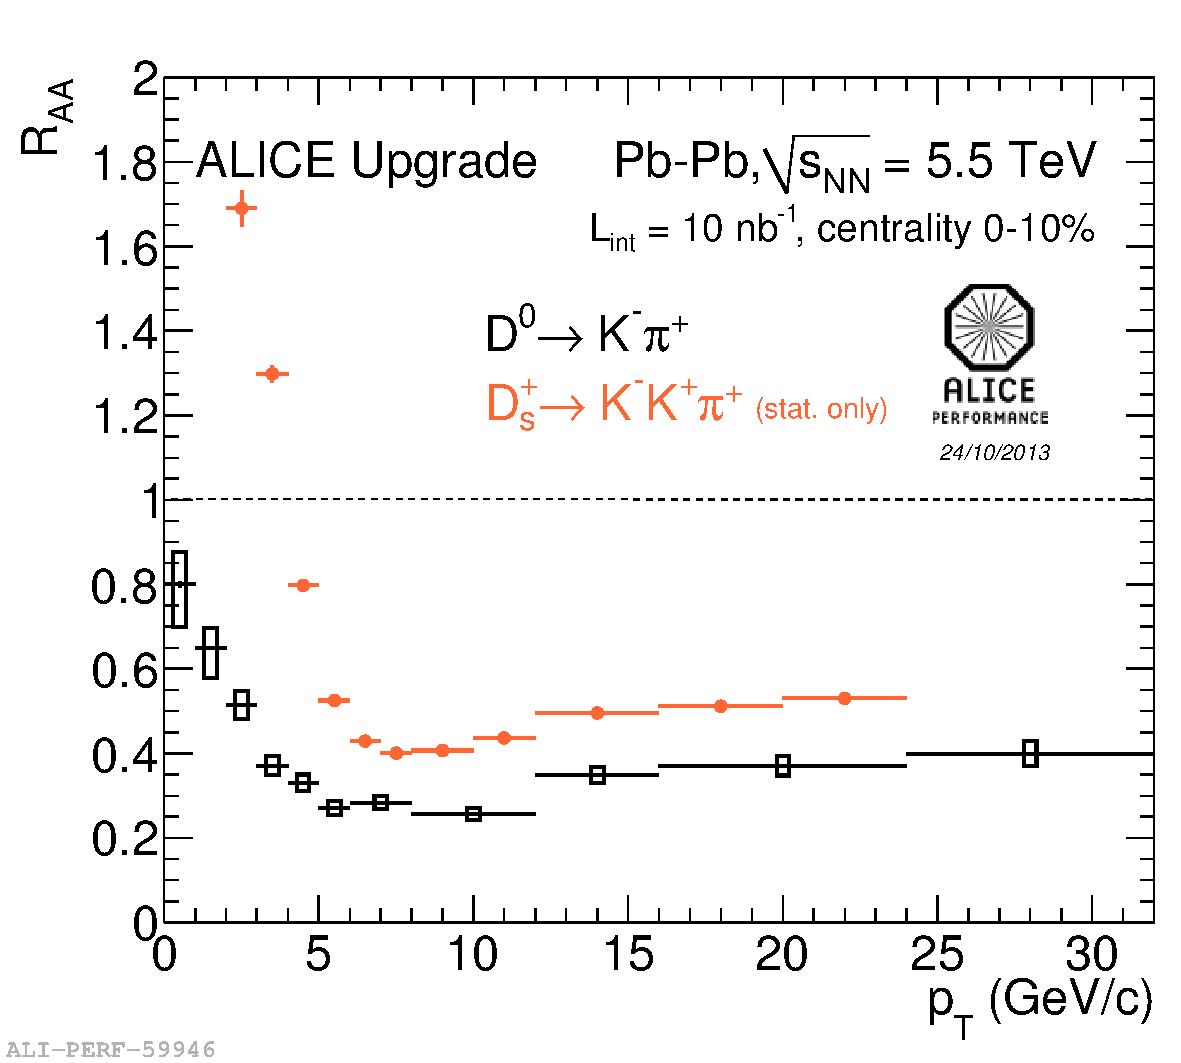
\includegraphics[width=0.49\textwidth]{hf/figures/2013-Oct-24-D0DsRAAprompt_TDR_logo.pdf}
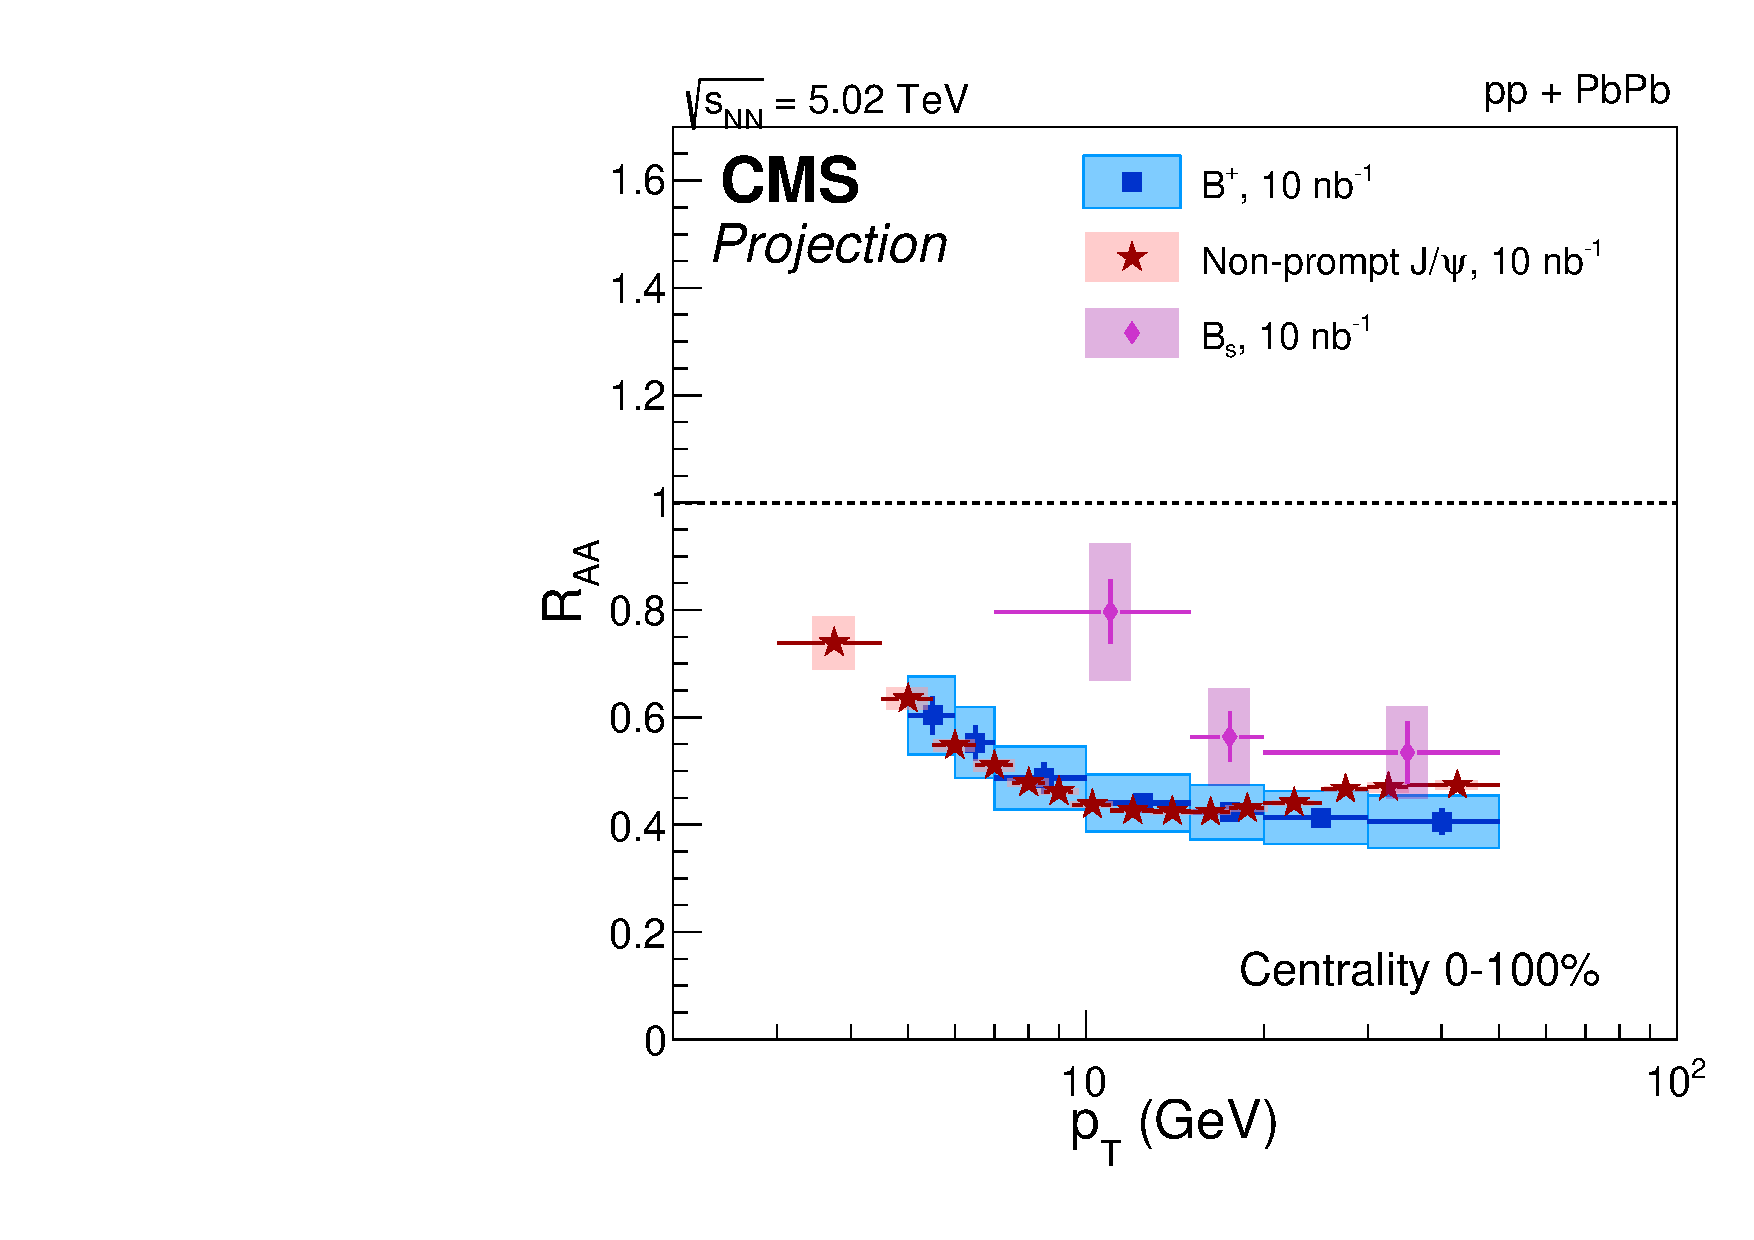
\includegraphics[width=0.45\textwidth]{hf/figures/CMS_B_Bs_RAA.pdf}
\caption{{\bf PLACEHOLDER: update/add systematics.} Measurement performance projections for the nuclear modification factor  $R_{\rm AA}$ of $D_s$ (left) and $B_s$ (right) mesons in Pb--Pb collisions ($L_{\rm int }=10~{\rm nb}^{-1}$). The ALICE projection for $D_s$ is based on full simulation~\cite{ITSTDR}. The CMS projection is based on scaling of uncertainties from existing measurements~\cite{CMSFTR2017}.}
\label{fig:HFDsBs}
\end {figure}

Figure~\ref{fig:HFLcLb} shows the projected performance for the charm and beauty baryon-to-meson ratios as they can be measured by ALICE with $L_{\rm int}=10$~nb$^{-1}$~\cite{ITSTDR}. The measurements are compared with predictions based on various mechanisms for heavy-quark recombination in the medium~\cite{Catania,TAMU,Ko}.
Figure~\ref{fig:D0DsLcv2} shows the projected performance for the elliptic flow coefficient $v_2$ of $D^0$, $D_s$ and $\Lambda_c$ 
in semi-central Pb--Pb collisions~\cite{ITSTDR}. The precision of the $D_s$ $v_2$ should be sufficient to enable a significant comparison with $D^0$ and with model calculations, in which the 
observable is found to be sensitive to the interactions of $D$ mesons in the hadronic phase that characterises the late stages of the collision~\cite{RappDs}. 
The $\Lambda_c$ measurement is still statistics-limited with $L_{\rm int}=10~{\rm nb}^{-1}$, thus motivating studies for a further improvement of the ALICE inner tracker during LS3~\cite{ALICEITS3}.  A more precise measurement would open the possibility to test in the charm sector some features at present only observed for the $v_2$ of light-flavour hadrons: the mass scaling at low $\pt$ and 
the baryon--meson grouping at high $\pt$.


\begin{figure}[ht]
\centering
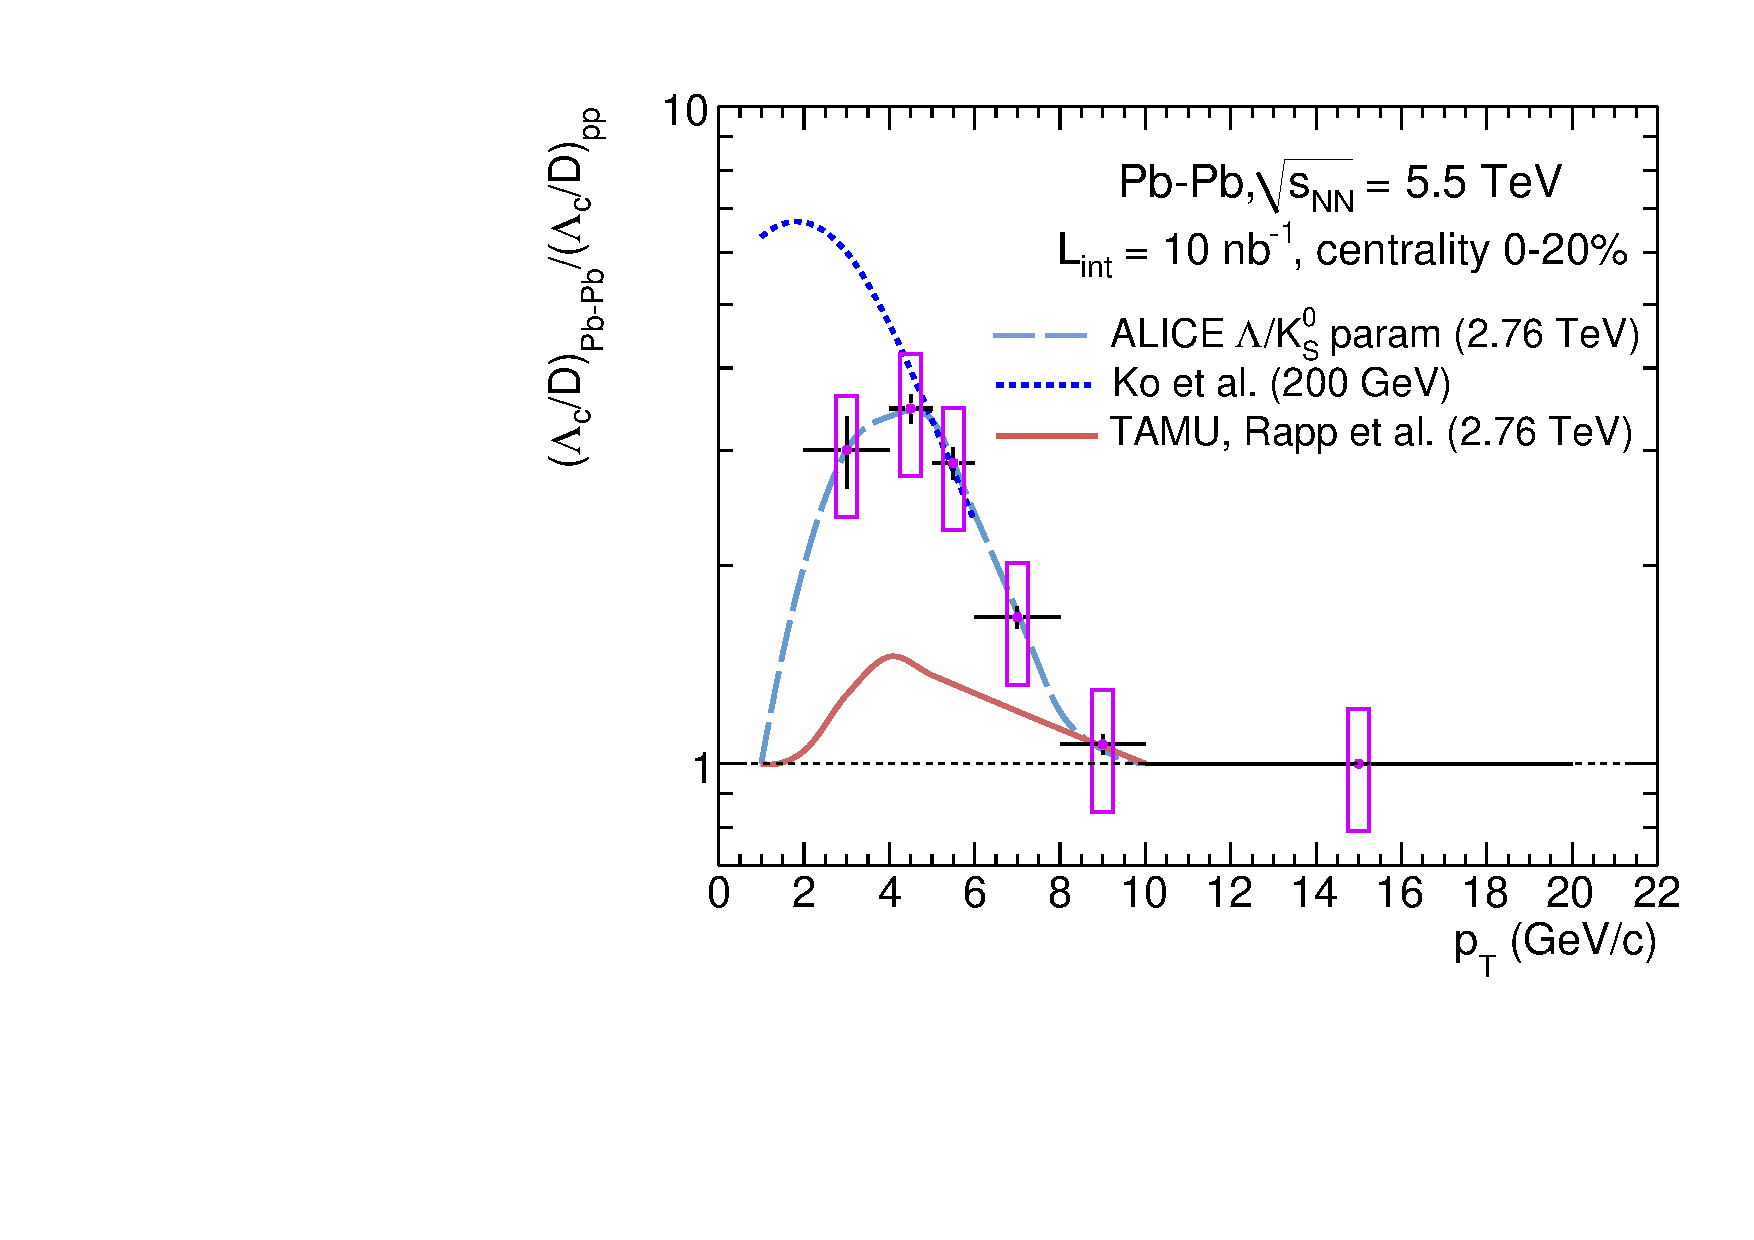
\includegraphics[width=0.49\textwidth]{hf/figures/LambdacOverD0_DoubleRatio_10nb_TDR.pdf}
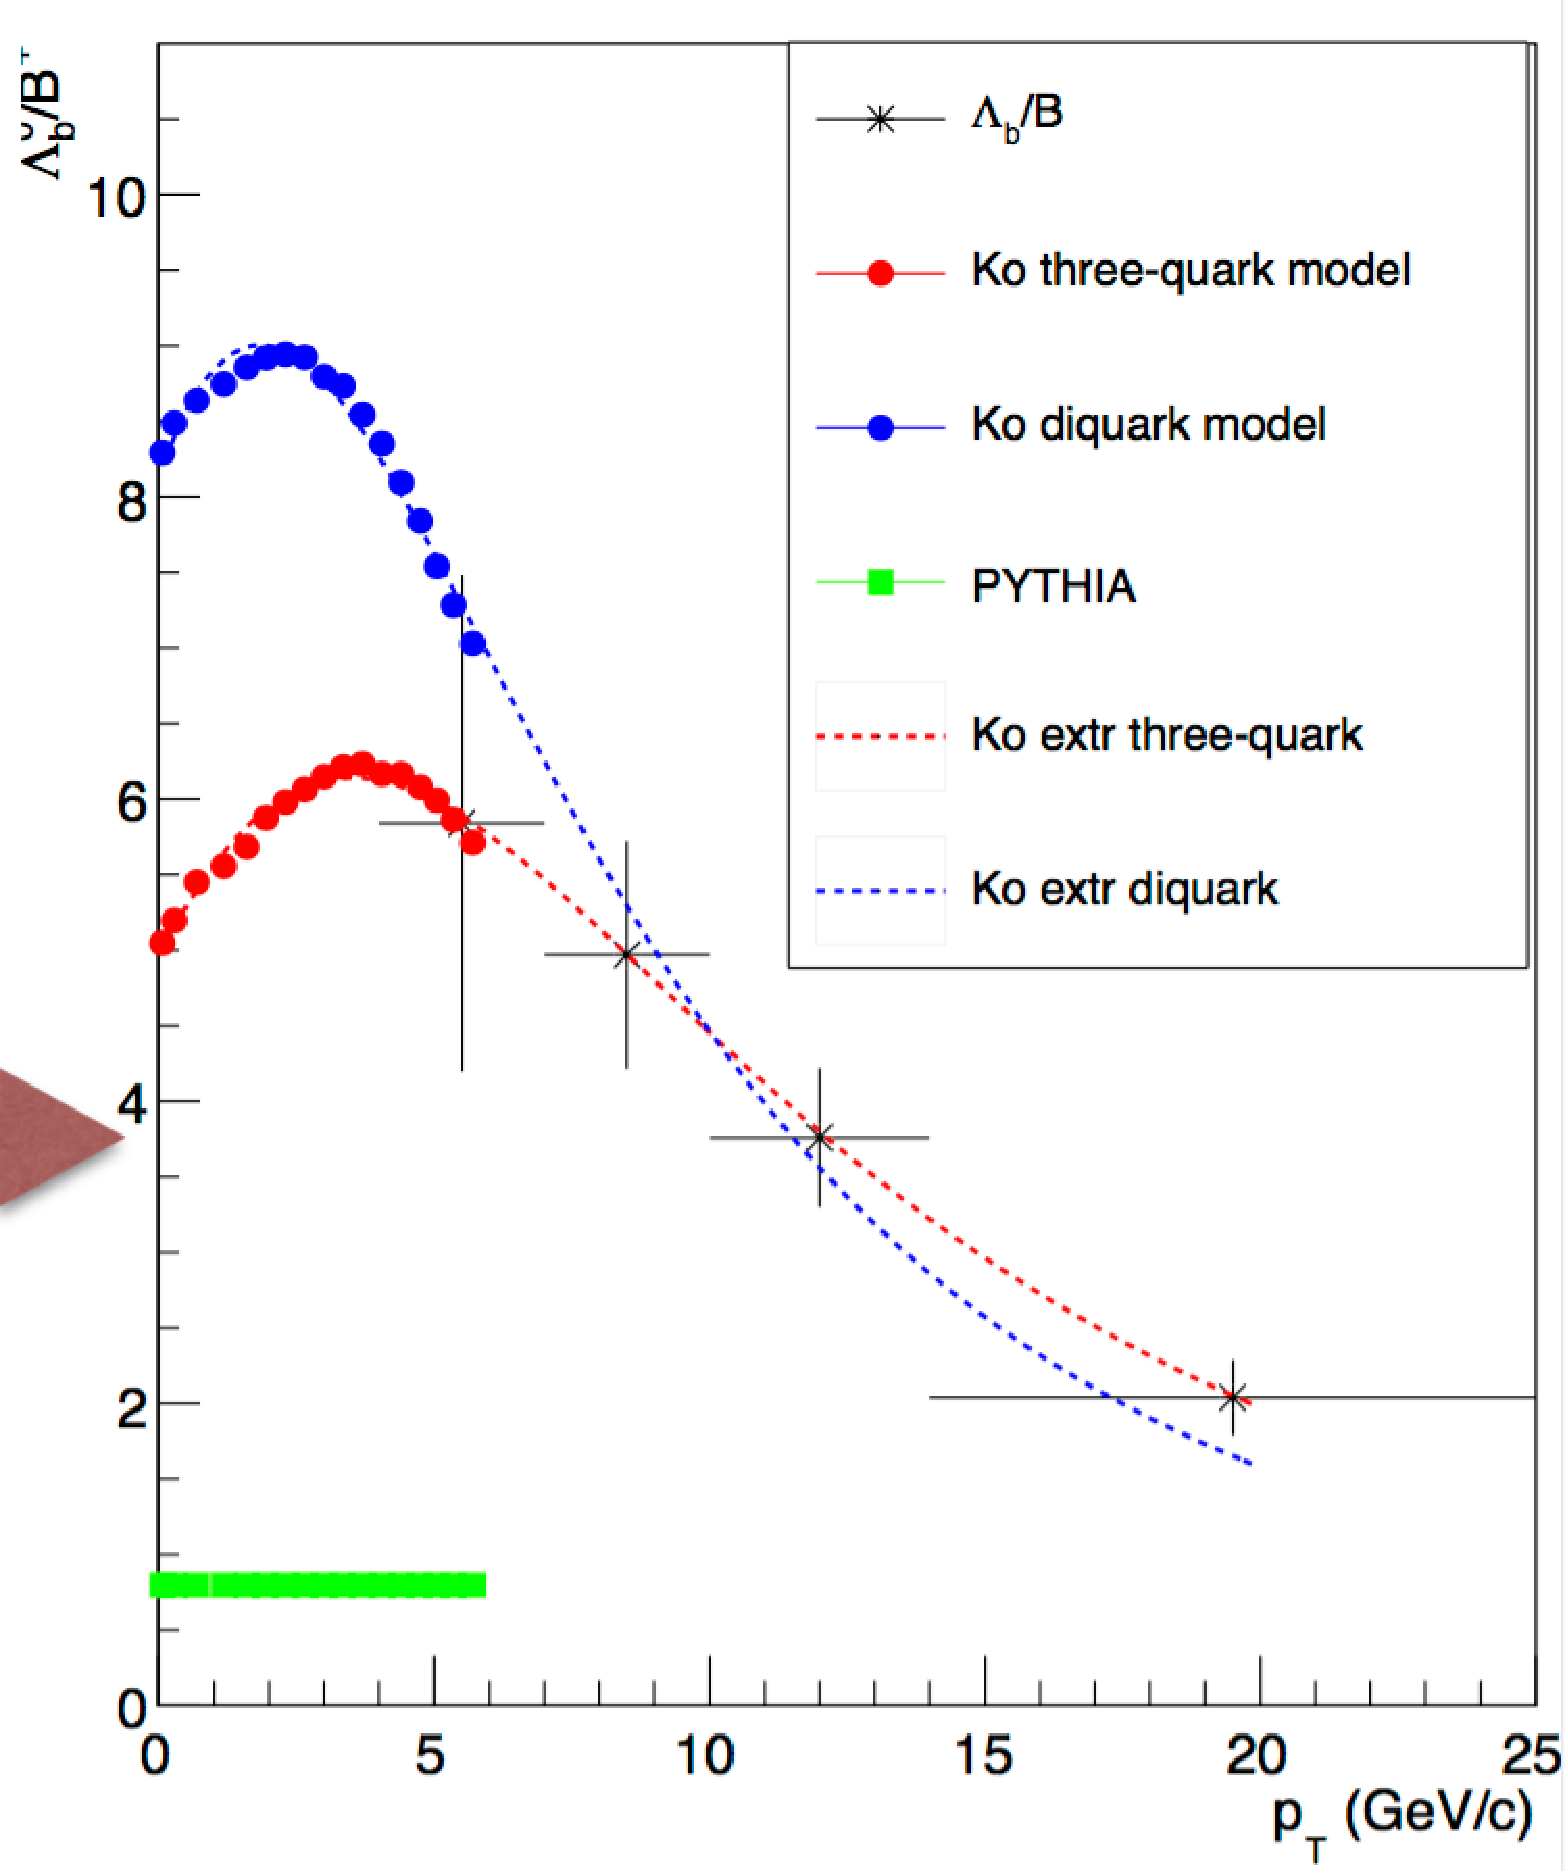
\includegraphics[width=0.39\textwidth]{hf/figures/LbOverB_tmp.pdf}
\caption{{\bf PLACEHOLDER: use PbPb only for Lc; official Lb figure.} ALICE measurement performance projections for the $\Lambda_c/D^0$ (left) and $\Lambda_b/B^+$ ratio in central Pb--Pb collisions ($L_{\rm int }=10~{\rm nb}^{-1}$), based on studied from~\cite{ITSTDR}.}
\label{fig:HFLcLb}
\end {figure}




\begin{figure}[ht]
\centering
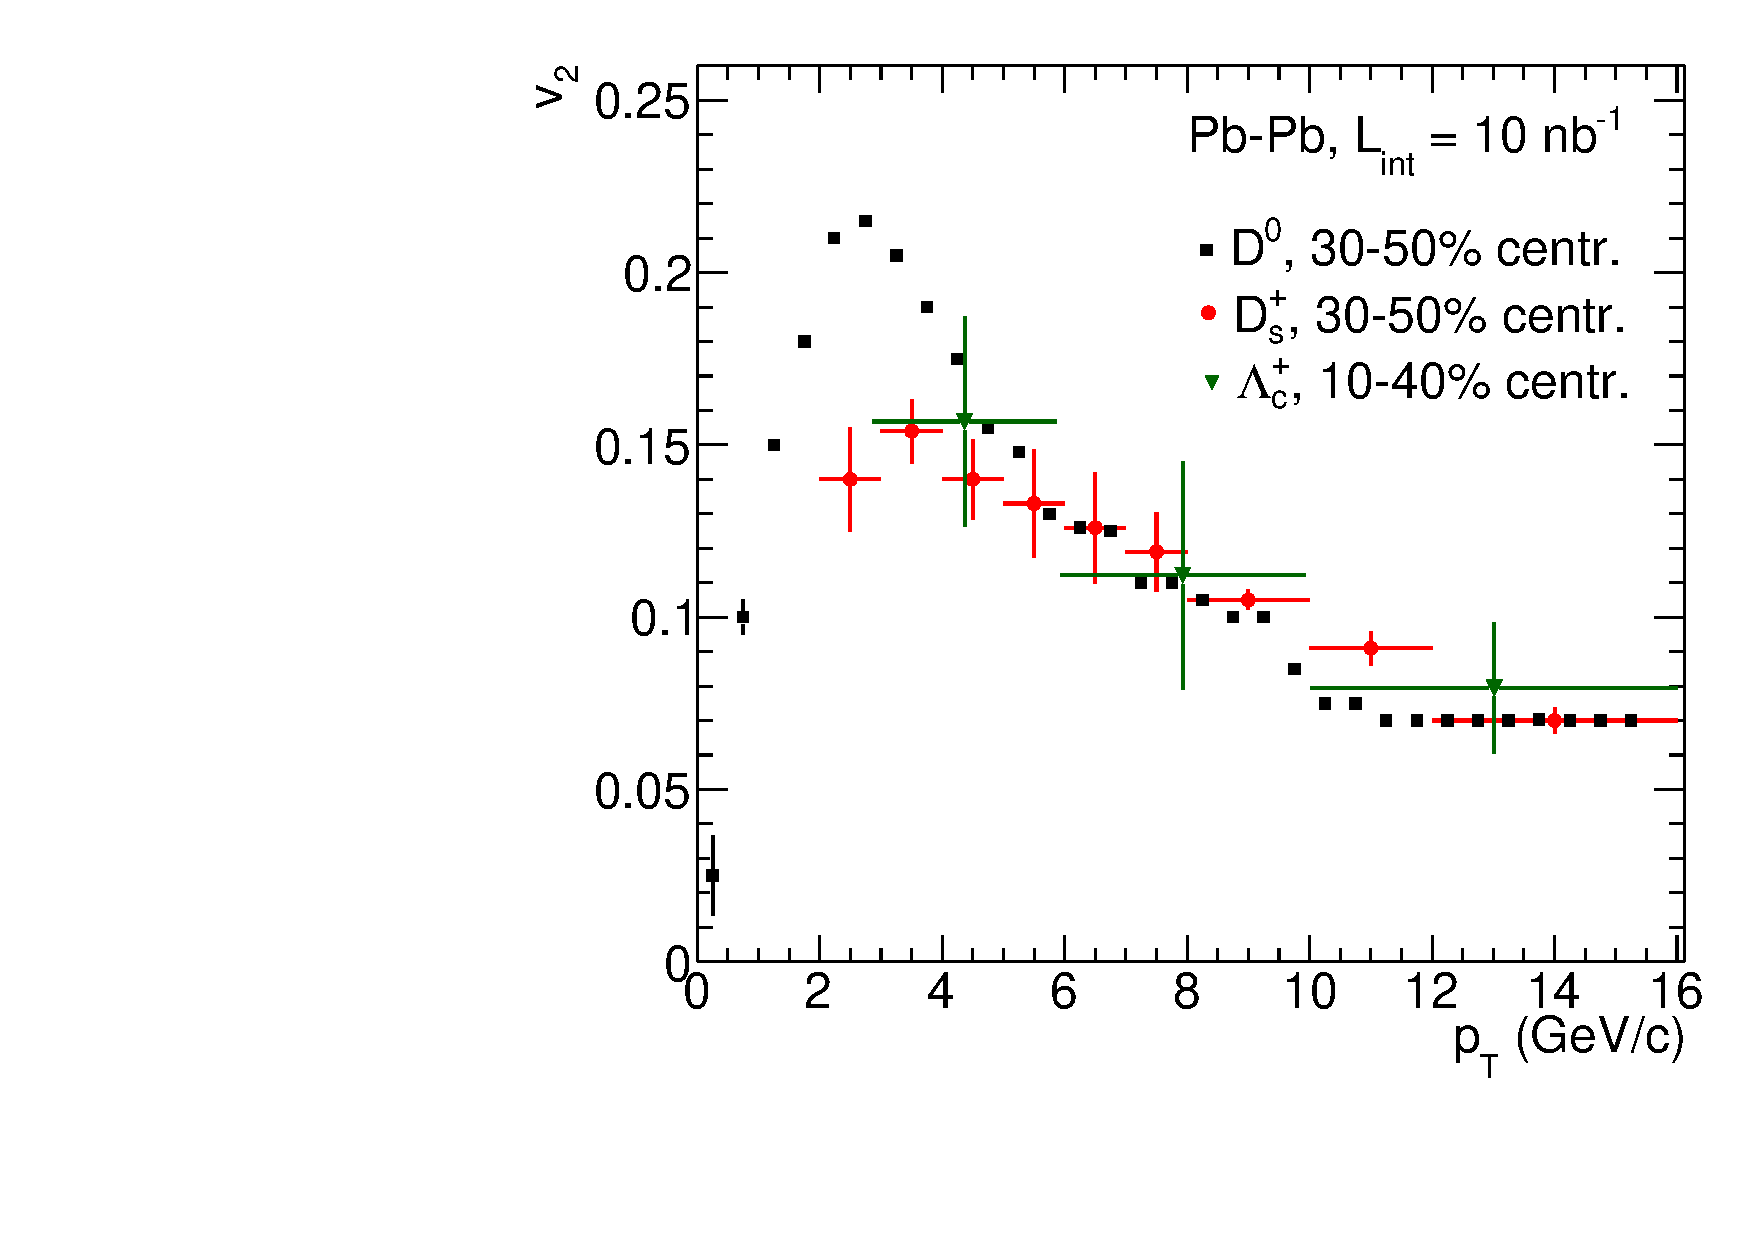
\includegraphics[width=0.40\textwidth]{hf/figures/D0DsLc_v2_TDR.pdf}
\caption{ALICE measurement performance projections for the elliptic flow coefficient $v_2$ of $D^0$, $D_s$ and $\Lambda_c$ in Pb--Pb collisions ($L_{\rm int }=10~{\rm nb}^{-1}$)~\cite{ITSTDR}.}
\label{fig:D0DsLcv2}
\end {figure}



\subsubsection{Constraining HF hadronization}

Discuss sensitivity of expected measurements to recombination fraction and parameters (use Catania model as example)

Discuss impact on extraction of HQ diffusion coefficient

Figure?
